\documentclass[letterpaper,11pt]{article}
\usepackage[spanish]{babel}
\usepackage[utf8]{inputenc}
\usepackage{graphicx}
\DeclareGraphicsExtensions{.jpg,.pdf,.mps,.png}
%Paquetes adicionales, ayudan para portada (algunos)
\usepackage{amssymb}
\usepackage{amsfonts}
\usepackage{amsmath}
\usepackage{fancyhdr}
\usepackage{wrapfig}
\usepackage[dvipsnames]{xcolor}
\colorlet{LightRubineRed}{RubineRed!70!}%https://www.overleaf.com/learn/latex/Using_colours_in_LaTeX
\usepackage{multicol}
\usepackage{changepage}
\usepackage{float}
\usepackage{tcolorbox}
\usepackage{enumitem}
%https://tex.stackexchange.com/questions/455341/how-to-represent-the-shift-key
%https://tex.stackexchange.com/questions/176398/carriage-return-symbol-new-command
\usepackage{keystroke}
\usepackage{menukeys}
\usepackage{tabularx,ragged2e,booktabs,caption}
\definecolor{gray51}{rgb}{0.51,0.51,0.51}


% Márgenes
\usepackage[vmargin=1.5cm,hmargin=2cm,head=30pt,includeheadfoot]{geometry}

% Interlineado
\linespread{1.5}
\usepackage{hyperref}
\usepackage{natbib}
\setcitestyle{super}
\usepackage{blindtext}
\linespread{1.0}\selectfont

% Definir estilo fancy
% Encabezado
\fancypagestyle{style1}{
\fancyhf{}
\lhead{
  \begin{wrapfigure}{l}{0.2\textwidth}
    \vspace{-0.69cm}
    \noindent \hspace{-1.10cm} 
\includegraphics[scale=0.2]{logos_dcc/logo_fac/fcfm_dcc_png}
  \end{wrapfigure}
  \hspace*{0.3cm}
  \textcolor{RubineRed}{\textsf{Liceo 1 Javiera Carrera}} \\
  \hspace*{0.3cm}
  \textcolor{gray51}{\textsc{Resumen Probabilidad N$^{o}$1}}} % Licencia en la izquierda del encabezado
\rhead{} % Logo
\fancyfoot{}
\renewcommand{\headrulewidth}{0.4pt}
}


\fancypagestyle{style2}{
\fancyhf{}
\lhead{
\begin{wrapfigure}{l}{0.2\textwidth}
\vspace{-2.4cm}

\includegraphics[scale=0.2]{fcfm_dcc_png}
\end{wrapfigure}
  %\hspace*{0.3cm}
  %\textcolor{RubineRed}{\textsf{Liceo 1 Javiera Carrera}} \\
  %\hspace*{0.3cm}
  %\textcolor{gray51}{\textsc{Resumen Probabilidad N$^{o}$1}} % Licencia en la izquierda del encabezado
  %\vspace{0.6cm}
} % TITULO DEL ENSAYO
\rhead{\textsf{Universidad de Chile\\ Departamento de Ciencia de la Computación}\\
\textbf{\textsf{Modelacion y Comp. Gráfica CC3501}}
\vspace{0.1cm}}
\renewcommand{\headrulewidth}{0.4pt}
}


\begin{document}

\pagestyle{style2}
\begin{figure}
\centering
\begin{minipage}[c]{0.8\textwidth}
\centering
\vspace{0.3cm}
{\large Informe de documentación}\\
{\Large Visualizador de Edificios}
\vspace{0.3cm}\\
Profesor: Daniel Calderón\\
Fecha: \today\\
Autor: Sebastián Sepúlveda A.
\end{minipage}
\end{figure}

{\centering \textbf{{\Large Resumen}}}\\

El presente documento presenta una breve descripción del trabajo y los pasos realizados para la elaboración de un \textit{visualizador de edificios} empleando técnicas proyecciones, texturas y curvas. El edificio que se escogió modelar fue Willis Tower, Chicago, Estados Unidos, y los objetivos que se lograron cumplir fueron practicar el uso de OpenGL para figuras en 3D, aplicar los conceptos de modelado de objetos en 3D y entender el uso de texturas y cámaras.\\

{\centering \textbf{{\Large Cámara}}}\\

\begin{wrapfigure}{r}{0.4\textwidth}
  \centering
  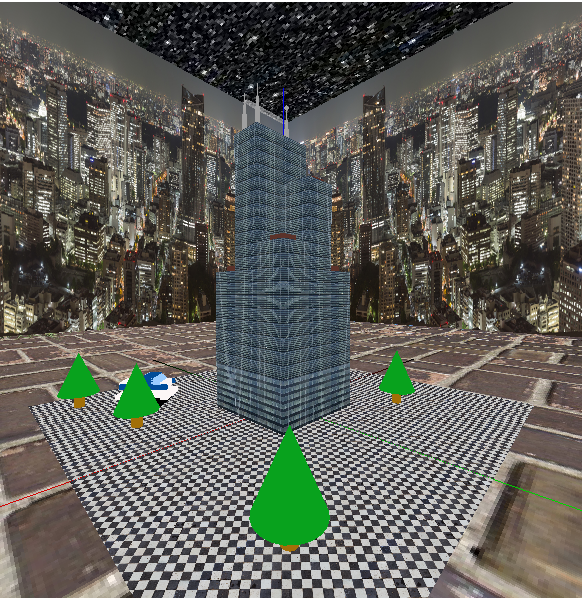
\includegraphics[scale=0.45]{images/tarea2/vista_periferica_tower.png}
  \captionof{figure}{Vista inicial de la cámara}
  \label{fig: vista_inicial}
\end{wrapfigure}

En el comienzo de la elaboración del programa fue necesario implementar las funciones necesarias para lograr diseñar una cámara que fuera cómoda de manejar y rápida en el movimiento a distintos lugares del espacio del escenario. La implementación de la cámara se hizo con la ayuda del concepto de \textit{Ángulos de Euler}, los cuales son bastante útiles para las rotaciones que se realizan en la cámara, y generan un mejor efecto en la vista de ``helicóptero'' que se esperaba realizar. Además del concepto anterior, también se modificó la vista de cámara con la ayuda de la vista perspectiva, que al variar el \textit{ángulo de fovia} genera un efecto de alejamiento y acercamiento útil para no utilizar solamente la modificación de los valores de \texttt{EYE} y \texttt{AT} en la matriz \texttt{LookAt}, que al abusar de su uso, puede generar efectos de \texttt{Cliping} indeseados, como la desaparición de cuerpos en la vista.

La implementación de las cámaras estáticas, se resolvió modificando los vectores de \texttt{EYE} y \texttt{AT} y estableciéndolos fijos según la tecla presionada, manteniendo el estado hasta que el usuario no presione el botón de desactivación de la vista estática. El desafió no fue complicado, pero fue necesario establecer una configuración manual para cada vista distinta. En la \textbf{Figura 1} se observa la vista inicial del programa, la cual no es una cámara estática.

El tiempo dedicado para completar la funcionalidad completa de la cámara fue de 6 horas, dividas en 3 días, debido a errores y ajustes en la vista de la cámara.\\

{\centering \textbf{{\Large Edificio y entorno}}}\\

El edificio que se escogió, como se mencionó anteriormente: \textit{Willis Tower, Chicago}, se realizó vía cubos con textura, con variadas traslaciones y repeticiones en el proceso para lograr un acercamiento con la realidad. El calculo de varios cubos gasta bastante memoria, por lo que se ignoró este problema y se priorizó la presentación por sobre la eficiencia. Para los detalles del edificio, como las antenas, los ventiladores ubicados en la planta alta y el entorno del edificio, se realizaron nuevas figuras, modificando  el archivo \texttt{basic\_shapes.py} y añadiendo conos, cilindros, esferas. La dificultad mayor se tuvo con el cono y la esfera. El cono se resolvió con la unión de los puntos de dos circunferencias paralelas, y la esfera se logró diseñar con la ayuda de las coordenadas esféricas y de paralelos y meridianos, como el globo terráqueo.

\begin{wrapfigure}{l}{0.4\textwidth}
  \centering
  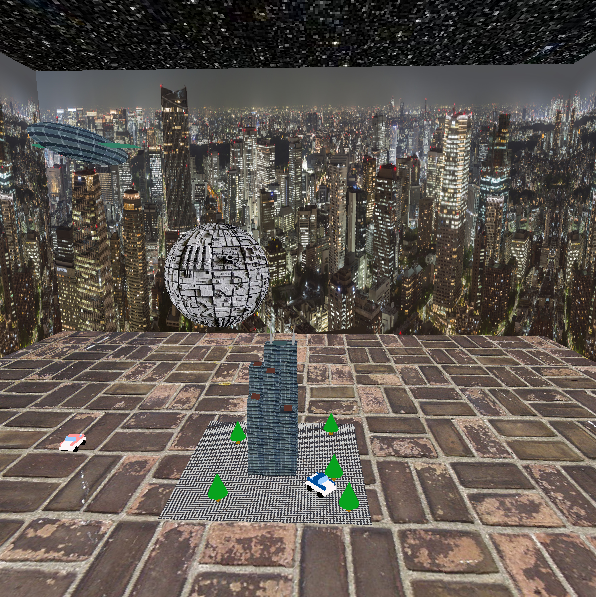
\includegraphics[scale=0.45]{images/tarea2/ciudad_entera.png}
  \captionof{figure}{Vista general mundo. Entorno completo del edificio}
  \label{fig: vista_inicial}
\end{wrapfigure}

Para el entorno del edificio se realizaron 4 cuerpos: \texttt{Árbol}, \texttt{Avión}, \texttt{Suelo y Cielo}, y \texttt{Auto}. Para los arboles, se hizo un modelo simple de un pino, con un cono como hojas y un cilindro de tallo. El Suelo y Cielo se realizaron con un cubo lo suficientemente grande para abarcar la vista de la cámara, con textura de ciudad para simular el suelo y los lados, y un plano para el cielo, con textura de estrellas, para simular un ambiente de ciudad nocturna. Para el auto se reutilizó el diseño visto en auxiliar para un auto, junto con la animación de un movimiento círculos alrededor del edificio. El avión se realizó con la ayuda de una esfera con textura y 2 alas, creadas con la ayuda de una superficie de \texttt{Catmull Roll} creada en auxiliar. El avión sigue una trayectoria según una curva de \texttt{Hermite}, cuyos parámetros de los puntos están fijos y no se pueden modificar por el usuario. En la \textbf{Figura 2} es posible observar la vista general del mundo creado.

Las mayores dificultades en la creación del entorno fueron las configuraciones que se debía realizar a cada objeto por separado para que estuviera en una posición adecuada y con un ajuste lo suficientemente adecuado para mantener una estética y orden en el programa.

El tiempo que dedicado a esta parte fue el más largo de todos los procesos, debido a la cantidad de objetos creados y a la dificultad para crearlos como se menciona. Entre 5-6 horas por día, por 3 días se dedicó a este proceso.

\textit{Extra:} Se realizó también la estrella de la muerte con la ayuda de la esfera con textura. Es posible visualizarla presionando \texttt{KEY G}, y aparece en conjunto con el avión.\\


%\begin{wrapfigure}[NÚMERO LÍNEAS]{POSICIÓN}[OVERHANG]{ANCHO}
% Insertar imagen
%\end{wrapfigure}


{\centering \textbf{{\Large Instrucciones de ejecución:}}}
\\
\texttt{ESPACIO:} Muestra/oculta lineas que generan la figura\\
\texttt{KEY LEFT CONTROL}: Muestra/oculta los ejes del plano. Por defecto oculta\\
\texttt{KEY G:} Cambia la forma del escenario, de cúbica a esférica \\
\textbf{\texttt{KEY 1, 2, 3, 4:}} Cambia la posición de la cámara a distintos puntos, con la cámara siempre paralela al edificio. Para volver a la camara movil es necesario presionar \texttt{KEY RIGHT CONTROL.}\\
\texttt{DESPLAZAMIENTO DE MOUSE:} Mueve el "ojo" de la cámara dependiendo de cuanto se desplace el mouse.\\
\texttt{SCROLL MOUSE:} Aleja/acerca el ángulo de fobia de la vista en perspectiva, generando un efecto de zoom.\\
\texttt{KEY ESC:} Salir del programa\\
\texttt{KEY O:} Muestra/oculta "Death Star" y avión que sigue trayectoria según curva de Bezier cerrada.\\
\\
\textbf{PRECAUCIÓN:} Si se mueve el mouse durante la cámara estática, la vista de la cámara movil será afectada. Se asume que el usuario sólo presionará los botones sin otras acciones.

\end{document}
